% !TEX TS-program = pdflatex
% !TEX encoding = UTF-8 Unicode

% This is a simple template for a LaTeX document using the "article" class.
% See "book", "report", "letter" for other types of document.

\documentclass[11pt]{article} % use larger type; default would be 10pt

\usepackage[utf8]{inputenc} % set input encoding (not needed with XeLaTeX)

%%% Examples of Article customizations
% These packages are optional, depending whether you want the features they provide.
% See the LaTeX Companion or other references for full information.

%%% PAGE DIMENSIONS
\usepackage{geometry} % to change the page dimensions
\geometry{a4paper} % or letterpaper (US) or a5paper or....
% \geometry{margin=2in} % for example, change the margins to 2 inches all round
% \geometry{landscape} % set up the page for landscape
%   read geometry.pdf for detailed page layout information

\usepackage{graphicx} % support the \includegraphics command and options

% \usepackage[parfill]{parskip} % Activate to begin paragraphs with an empty line rather than an indent

%%% PACKAGES
\usepackage{booktabs} % for much better looking tables
\usepackage{array} % for better arrays (eg matrices) in maths
\usepackage{paralist} % very flexible & customisable lists (eg. enumerate/itemize, etc.)
\usepackage{verbatim} % adds environment for commenting out blocks of text & for better verbatim
\usepackage{subfig} % make it possible to include more than one captioned figure/table in a single float
% These packages are all incorporated in the memoir class to one degree or another...

%%% HEADERS & FOOTERS
\usepackage{fancyhdr} % This should be set AFTER setting up the page geometry
\pagestyle{fancy} % options: empty , plain , fancy
\renewcommand{\headrulewidth}{0pt} % customise the layout...
\lhead{}\chead{}\rhead{}
\lfoot{}\cfoot{\thepage}\rfoot{}

%%% SECTION TITLE APPEARANCE
\usepackage{sectsty}
\allsectionsfont{\sffamily\mdseries\upshape} % (See the fntguide.pdf for font help)
% (This matches ConTeXt defaults)

%%% ToC (table of contents) APPEARANCE
\usepackage[nottoc,notlof,notlot]{tocbibind} % Put the bibliography in the ToC
\usepackage[titles,subfigure]{tocloft} % Alter the style of the Table of Contents
\renewcommand{\cftsecfont}{\rmfamily\mdseries\upshape}
\renewcommand{\cftsecpagefont}{\rmfamily\mdseries\upshape} % No bold!

%%% END Article customizations

%%% The "real" document content comes below...

\title{Sternenkrieg}
\author{Christian Bauer\\ xyz@edu.aau.at
\and Lukas Pagitz \\ xyz@edu.aau.at
\and Anja Ressmann \\ xyz@edu.aau.at
\and Christoph Roither \\ xyz@edu.aau.at
\and Boda Wen \\ xyz@edu.aau.at}
\date{21.06.2017}

% Eigene Änderungen
\usepackage[ngerman]{babel} % Silbentrennung
\setlength\parindent{0pt} %  keine Einrückung
\usepackage{graphicx}
\usepackage{float}
\usepackage[autostyle=true,german=quotes]{csquotes}
\usepackage{hyperref}

\begin{document}
\maketitle

\begin{center}
Software Engineering II - SS 16/17

\hfill \break

Univ.-Prof. Dipl.-Ing. Dr. Martin Pinzger

Univ.-Ass. Dipl.-Ing. Christian Macho

\hfill \break
\\[3em]
\begin{figure}[H]
	\centering
 	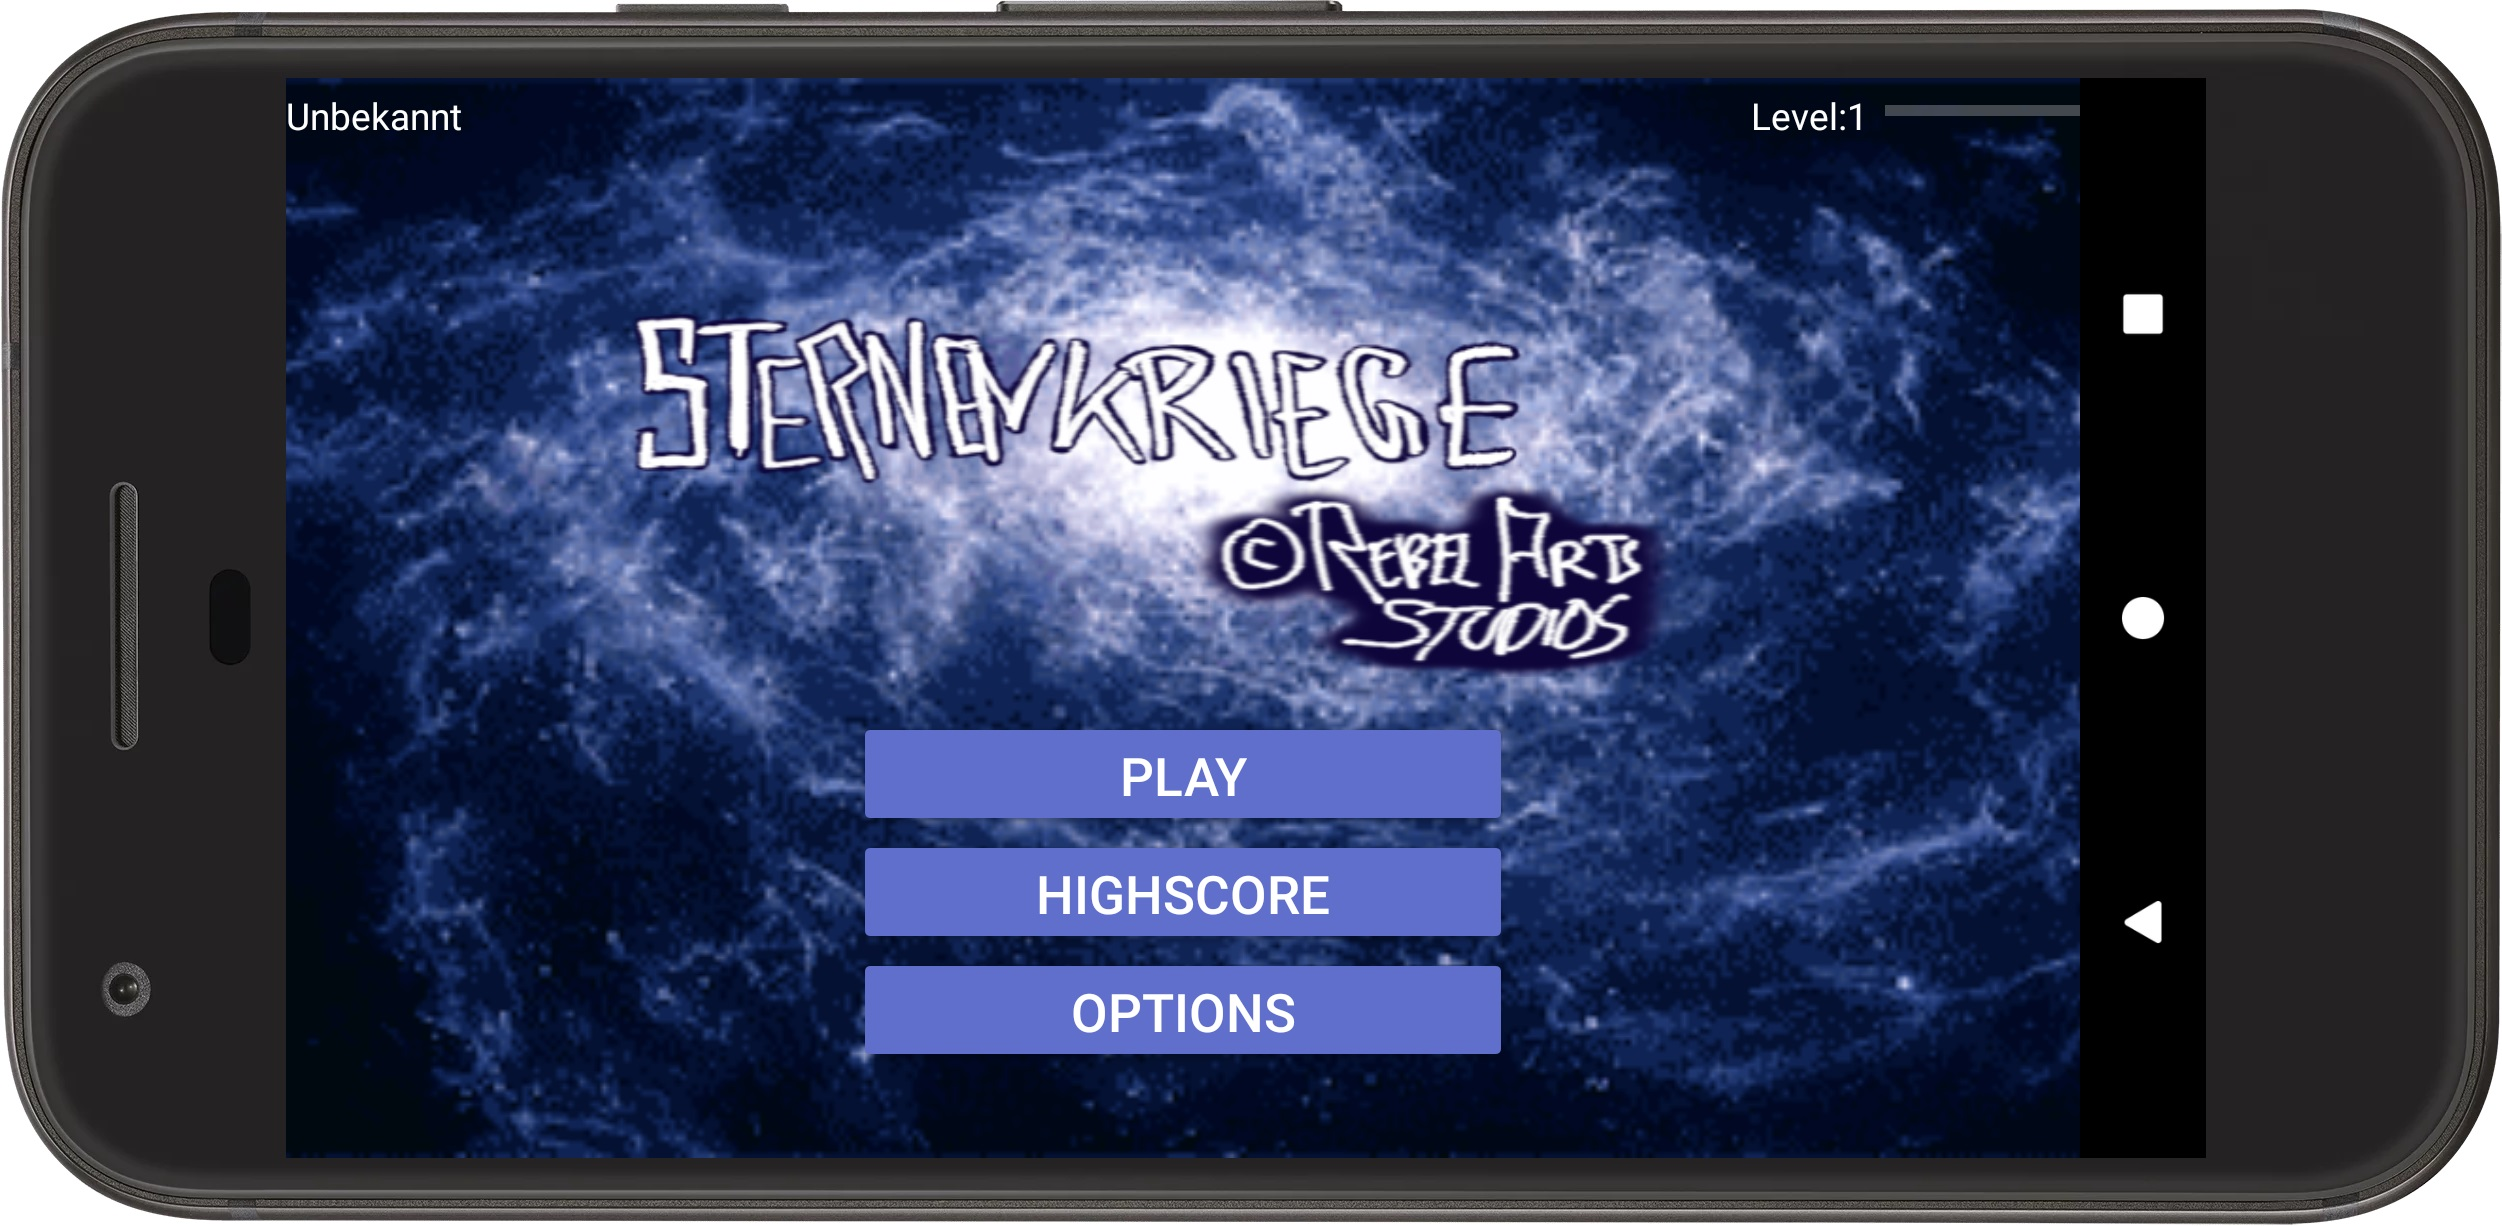
\includegraphics[width=1\textwidth]{img/main}
	\caption{Startbildschirm von Sternenkrieg}
\end{figure}
\end{center}
\hfill \break
\newpage
\tableofcontents

\newpage

\section{Einleitung}

Sternenkrieg <TODO>

\section{Grundlegender Aufbau}
\subsection{Spielablauf}
Sternenkrieg orientiert sich am Spielprinzip von "Schiffe versenken". Ziel ist es, die vom Gegner platzierten Schiffe als erster Spieler zu zerstören. Als Erweiterung zum herkömmlichen Spiel, bietet Sternenkrieg weitere Features, deren technische Funktionalität hier kurz erläutert wird. Dieses Kapitel soll zum Verständnis des Ablaufs im Programm beitragen.

Gestartet wird das Spiel mit einem Klick auf den Button "Play". Danach muss eine Verbindung zwischen beiden Spielern hergestellt werden. Hierzu ist es notwendig, dass sich die Smartphones beider Spieler im gleichen WLAN-Netzwerk befinden. Ein Spieler übernimmt im Spiel den Server, der andere übernimmt den Client.

Der Server-Spieler startet danach den Server und bekommt eine IP-Adresse angezeigt, welche er dem Client-Spieler übermittelt. Dieser verbindet sich damit zum Server. Sobald die Verbindung erfolgreich war, melden sich beide Spieler als bereit und das Spiel beginnt.

Um zu entscheiden, welcher der beiden Spieler das Spiel beginnen soll, muss gewürfelt werden. Dies geschieht durch Schütteln des Smartphones. Der Wert des jeweiligen Gegners wird dabei über das Netzwerk übertragen.

Nun beginnt das eigentliche Spiel: Jeder Spieler muss seine Schiffe (ein kleines, ein mittleres und ein großes) platzieren. Ziel des Gegners ist es nun, die Schiffe des Gegners zu zerstören, bevor die eigenen vernichtet werden.

Im weiteren Spielverlauf werden auch die besonderen Features von Sternenkrieg sichtbar. Diese sind unter anderem eine Schummelfunktion sowie ein PowerUp-System.

\subsection{Menüaufbau}
Das Menü von Sternenkrieg bietet - abgesehen vom eigentlichen Spiel - noch folgende Buttons:
\begin{itemize}
\item Highscore -- zeigt den Highscore von Sternenkrieg an
\item Optoins -- öffnet die Einstellungen des Spiels
\item About -- zeigt eine kurze About Us-Meldung an
\end{itemize}


\section{Klassen im Überblick}
In diesem Kapitel werden die allgemeinen Klassen und die dazugehörigen Activities von Sternenkrieg beschrieben. Besonders wichtige Klassen und Methoden werden ausführlicher behandelt.

\subsection{About}
Die Klasse "About" gibt einen kurzen Text über Sternenkrieg aus und hat sonst keine weitere Funktionalitäten.

\subsection{Dice}
Die Klasse "Dice" steht einen Würfel zur Verfügung. Dieser Würfel wird am Beginn des Spiels verwendet um den Beginner des Spiels zu bestimmen. Der Würfel wird außerdem bei den PowerUps verwendet, um eine Zufallszahl zu erhalten.
Das Würfeln erfolgt durch Schütteln des Smartphones. Hierfür wird ein SensorEvent-Listener verwendet. Unterstützt wird die Klasse Dice durch die Klasse res/Sensors.

\subsection{DiceClass}

\subsection{HighScore}

\subsection{Main}
Die Klasse "Main" stellt den Startscreen sowie das Hauptmenü dar. Eingebunden werden hier das Hintergrundbild sowie die Buttons zur Menüauswahl. Falls das Spiel zum ersten Mal gestartet wird, muss vom Spieler ein Name eingegeben werden.

\subsection{MainSocket}

\subsection{Map}

\subsection{MapLoad}

\subsection{Options}
Die Klasse "Options" behandelt alle Einstellungsmöglichkeiten von Sternenkrieg. Dazu zählen:
\begin{itemize}
\item Name
\item Sound an/aus
\item Sprache (DE/EN)
\end{itemize}
Die Speicherung der Einstellungen erfolgt mithilfe von SharedPreferences ("prefs"). Diese bieten eine einfache Speicherung von Variablen, welche ebenfalls sehr einfach aktualisiert werden können. Nach einer Änderung wird die entsprechende Variable neu abgespeichert und steht somit auch den anderen Klassen zur Verfügung.

\subsection{PlayAudio}

\subsection{PowerUp}

\subsection{Spielfeld}

\section{GameLogic-Klassen im Überblick}
In diesem Kapitel werden die GameLogic-Klassen näher erläutert. Wie der Name schon sagt, beinhalten diese Klassen die eigentliche Spiellogik.

\subsection{GameUtilities}
Die Klasse "GameUtilities" verwaltet das Speichern der Informationen zum Spiel, darunter:
\begin{itemize}
\item Fortschritt
\item Highscore
\item Level
\item Sound an/aus
\item Username
\end{itemize}

Diese Informationen werden in den Shared Preferences "prefs" gespeichert. 

Die Klasse bietet unter anderem folgende Methoden:
\begin{itemize}
\item ArrayList<String> getHighscore() - liefert den aktuellen Highscore
\item void setHighscore() - setzt den aktuellen Highscore
\item void deleteHighscore() - löscht den Highscore

\item String getUsername() - liefert den gespeicherten Namen des Spielers
\item void setUsername(String username) - setzt einen neuen Namen (beim Start des Spiels bzw. in den Optionen)
\end{itemize}

\subsection{NetworkStats}

\subsection{PlayerFieldLogic}
In der Klasse "PlayerFieldLogic" wird die Logik des Spielfelds verwaltet. Die Spielfelddaten werden in einem String-Array gespeichert. Abhängig von den gespeicherten Informationen werden die Felder unterschiedlich gefärbt.

\subsection{PlayerFieldShipContainer}

\subsection{PlayerFieldValues}

\subsection{ShipLogic}

\section{Network-Klassen im Überblick}

\subsection{AcceptThread}

\subsection{Client1}

\subsection{Host}

\subsection{myhandler}

\subsection{NetworkUtilities}

\subsection{ReceiveThreadClient}

\subsection{ReceiveThreadHost}

\subsection{StartThread}

\subsection{WriteClient}

\subsection{WriteHost}

\section{Resources-Klassen im Überblick}

\subsection{QRReader}

\subsection{Sensors}

\section{Erklärung besonderer Funktionen}

\subsection{Shared Preferences}

\section{Zusammenfassung}

\end{document}
